\section{Clinical stratification} \label{clin}
% Note that this file describes only one implementation of the clinical stratification possible in the sm_sir code
The ``clinical" stratification acts by replicating each of the two age-stratified sequential compartments representing infectious COVID-19 into three categories.
The three clinical categories are:
\begin{enumerate}
    \item Asymptomatic persons
    \item Symptomatic persons who are never notified as cases
    \item Symptomatic persons who are successfully detected and notified
\end{enumerate}
For each age category, a proportion of new active infections are assumed to remain asymptomatic throughout their infectious period (specified in Table \ref{tab:age_params}).
This proportion remains fixed over time throughout a model run.
It is assumed that asymptomatic persons are never detected and so do not contribute to notifications.
The remaining proportion constitutes the second and third categories, comprising all persons developing symptomatic COVID-19 during their infectious period.
The proportion of these symptomatic persons who progress to the third category varies with time and is described under the section on case detection (Section \ref{cdr}).
\begin{figure}[ht]
    \begin{center}
    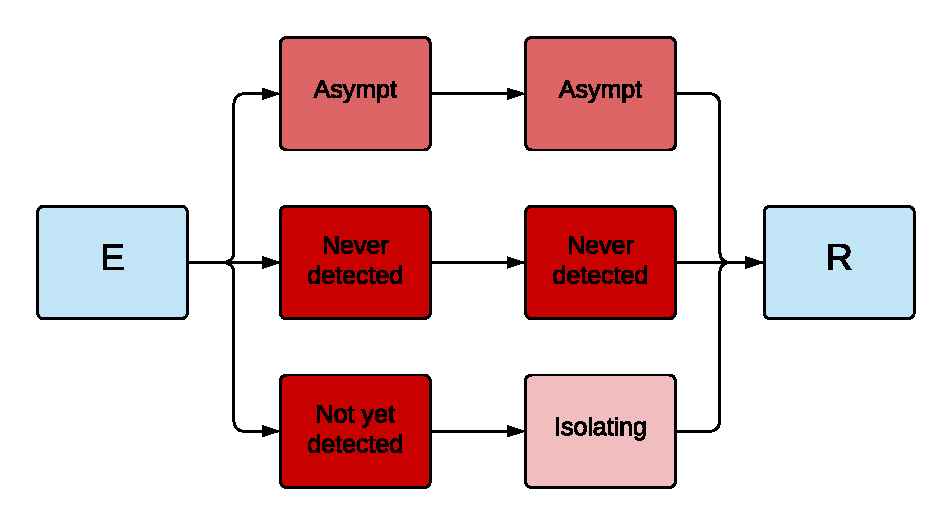
\includegraphics[width=0.7\textwidth]{../../tex_descriptions/models/sm_sir/stratifications/clinical_strat.pdf}
    \end{center}
    \caption{Illustration of the clinical stratification. \small Depth of red shading of compartment qualitatively indicates infectiousness.}
    \label{fig:seeiir}
\end{figure}